\section{Comparison with Dijkstra}\label{sec:comparison}

The Dijkstra algorithm tries to find a minimum \emph{spanning} tree which
contains links that connect a set of target nodes.

Differently from that, the minimum \emph{Steiner} tree considers for the
computations, to connect all the target nodes, also other nodes. So in this way
the lower bound of the optimal solution is less or equal than the result
provided by a \emph{spanning} tree algorithm (as we can see in
\figref{fig:steiner}). The price to pay is in term of time and computational
power, because the algorithm has to visit all the possible links and not the
subset that involves only the target nodes, so this solution has a limited
scalability.

\begin{figure}
	\centering
	\begin{subfigure}[b]{0.3\textwidth}
		\centering
		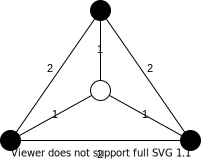
\includegraphics[width=\textwidth]{img/steiner-topology}
		\caption{An example of a network topology where black nodes are
		target nodes}\label{subfig:steiner-topology}
	\end{subfigure}
	\begin{subfigure}[b]{0.3\textwidth}
		\centering
		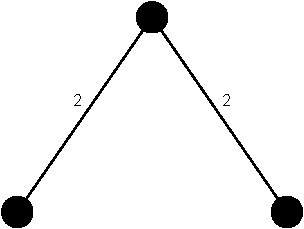
\includegraphics[width=\textwidth]{img/steiner-minspanning}
		\caption{The result of a minimum spanning tree algorithm on the
		example network topology. The result only contains links that
		involve target nodes. Its cost is
		4}\label{subfig:steiner-minspanning}
	\end{subfigure}
	\begin{subfigure}[b]{0.3\textwidth}
		\centering
		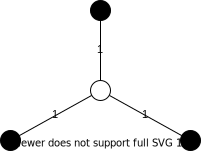
\includegraphics[width=\textwidth]{img/steiner-minsteiner}
		\caption{The result of a minimum Steiner tree algorithm on the
		example network topology. It includes also non-target nodes to
		build the tree. Its cost is 3}\label{subfig:steiner-minsteiner}
	\end{subfigure}
	\caption{An example of application of a minimum spanning tree algorithm
		and a minimum Steiner tree algorithm on the same
		topology}\label{fig:steiner}
\end{figure}
